% (c) 2020 Stefan Antonowicz
% Based off of tex found at https://github.com/ludus-leonis/nipajin
% This file is released under Creative Commons Attribution-NonCommercial-ShareAlike 4.0 International License.
% Please do not apply other licenses one-way.

\renewcommand{\yggCombat}{%
  \mychapter{Combat}{combat}
}

\renewcommand{\yggCombatText}{%
  \mysection{Rules of Engagement}{combat-rules}

  \mysubsection{Overview}{combat-overview}

  \mybullet {
    \item Combat is conflict that takes place between \mylink{Allies and Monsters}{combat-allies-monster} at a particular \mylink{Distance}{distance-combat}.

    \item Combat consists of \mylink{Moments}{time-combat} and takes \mylink{Minutes}{time-combat} to comple.  Each Moment consists of the Allies and Monsters taking a turn trying to resolve Combat.

    \item Each Moment you can perform \mylink{Actions}{combat-actions}.  You can take 1 or 2 Actions in a Moment. The number of Actions you can take depends on your \mylink{Init}{combat-init} roll.

    \item Actions are divided into two groups: Maneuver Actions and Combat Actions.  \mybold{If you take a Combat Action, your Moment ends}.

    \item Certain Actions occur at the \mylink{top and bottom of the Moment}{time-top-bottom}
  }



  \mysubsection{Allies and Monsters}{combat-allies-monsters}

  Allies consist of all the Adventurers and any henchmen or hirelings they might have;  Monsters are everyone (or everything) else involved in the Combat.  It could be a group of peasants armed with pitchforks, a timed trap, or a swarm of bees.  Could also be a monster.

  \mysubsection{Actions}{combat-actions}

  Combat consists of \mylink{Moments}{time-combat} and takes \mylink{Minutes}{time-combat} to finish.

  You can take 1 or 2 Actions in a Moment, depending on your \mylink{Initiative (Init)}{combat-init} roll. 

  If you \RO on your Init check, you can take 1 Action \mybold{before} the Monster and 1 Action \mybold{after} the Monster. If you fail, you can take 1 Action \mybold{after} the Monster. You can always choose to act after - there's no need to roll at that point. You can act as a group and decide your own order for Actions in each Moment. 

  \cbreak

  Your Actions can be:
  \mybullet {
    \item A Maneuver Action:  \mylink{Basic}{combat-basic-maneuver} or \mylink{Tactical}{combat-tactical-maneuver}, or;
    \item A Combat Action: \mylink{Fighting}{combat-fighting} or \mylink{Mighty Deed of Arms}{combat-mighty-deeds}
  }

  You can only take 1 Combat Action in a Moment, even if you win Init.


  \mysubsection{Initiative (Init)}{combat-init}

  To determine who goes first, all Allies roll their Init at the top of the Moment. The result of this \RO attempt will tell you how many Actions you can take.


  The Init check is a \RO attempt using the following dice:

  \example {
    \DEX \PLUS \MD \PLUS \mybold{Monster Speed}
  }

  \myhighlight{Move Die}{combat-move-die}

  Each type of armor has a \MD associated with it:

  \mytable{X r}{
    \thead{\mylink{Armor}{gear-armor}} & \thead{\MD} \\
  }{
    None & d20 \STATIC \\
    Light & d12 \STATIC \\
    Medium & d8 \STATIC \\
    Heavy & d4 \STATIC \\
  }

  \myhighlight{Move Die}{combat-monster-speed}

  Most Monsters have a speed of d16.  Some Monsters are Fast - their speed is d12.  Some Monsters are Slow - their speed is d20.  See the section on \mylink{Monsters}{bestiary} for more details.


  \myhighlight{Surprise}{combat-surprise}

  Before rolling Init the first time, the Arbiter will determine whether you or the Monster are surprised. Examples of surprise might be: attacking a group of goblins playing cards; someone kicking down the door and bum rushing you; a vampire fading in behind you and biting you in the neck; etc.

  If you are surprised at the start of Combat, you immediately lose Init. If you take damage in a Surprise Moment, it bypasses Grit.

  If a Monster is surprised at the start of Combat, all of the players automatically win Init.  Knaves can consider this getting "The Drop" on someone, meaning they can attempt a \mylink{Murder}{knave-murder}

  Knaves can also try to get the Drop on someone \myital{during} Combat.  More details can be found in the section on \mylink{Whispers: Gloomstride}{knave-whisper-gloomstride}. 

  \mysubsection{Maneuver Actions}{combat-maneuvers}

  A Maneuver Action does not end your Moment.  You may take a Maneuver as an Action.  



  \myhighlight{Basic Maneuvers}{combat-basic-maneuver}

  Basic maneuvers involve positioning yourself in combat, readying equipment, helping fallen Allies, etc.  A Maneuver is anything that might take you a handful of seconds to do.  For example:

  \mybullet { 
    \item Moving somewhere \mylink{Nearby}{distance-combat};  
    \item Readying a shield and/or weapon; 
    \item Switching weapons; 
    \item Picking up something you dropped; 
    \item Getting up from the Prone position; 
    \item Finding a spell in your grimoire; 
    \item Lighting a torch or flaming oil; 
    \item Grabbing something out of your pack; 
    \item Drinking a potion or applying a salve
  }

  Whether or not something qualifies as a Basic Maneuver is up to the Arbiter's discretion.  It's possible that an action might take longer than a single Maneuver.  Some examples:
  \mybullet {
    \item Picking a lock while a fight rages around you;
    \item Tying off a rope and swinging into combat;
    \item Running across the room and digging through a fallen Allies pack;
    \item etc.
  }

  The Arbiter should decide how many Actions this will take ("it'll take you an Action to tie off the rope and another Action to swing into Combat"; "it's an Action to move Nearby, another Action to roll him over and open his pack, and a third Action to find what you're looking for").

  \myhighlight{Tactical Maneuvers}{combat-tactical-maneuver}

  Tactical Maneuvers involve creating scenarios to positively influence your next Combat Action or change the environment of the battlefield.  They have a few rules:

  \mynumlist {
    \item You can only use one Tactical Maneuver at a time
    \item Unless it says otherwise, bonuses and penalties to Fight or Guard occur for a single \RO check
    \item Tactics don't stack i.e. you can't Aim for multiple Moments and stack the bonuses
  }


  \myhighlight{Aim}{combat-tactical-maneuver-aim}
  \myital{Shoot or Throw Weapons Only}
  
  You take careful aim with your weapon. Your \myital{next} Fight \RO gets a modifier of +4, but your Guard \RO gets a modifier of -4.  These modifiers lasts until you take a Combat Action or something breaks your aim (moving, taking damage, etc)

  \myhighlight{Block}{combat-tactical-maneuver-block}
  If you have an Action before the Monsters, you can move somewhere Nearby.  The Monster will attack you during its Action if \RS : Presence.

  \myhighlight{Brace}{combat-tactical-maneuver-brace}
  \myital{Polearm or spear only}
  If a Monster moves Close to you during its turn, you may immediately take a Combat Action \mybold{before} the Monster attacks

  \myhighlight{Rage}{combat-tactical-maneuver-rage}
  You take an Action to be come \mylink{Enraged}{effect-enraged}.  The target of the rage is "the Monsters". If one of your Allies has injured you in this fight, they count as a Monster.

  \myhighlight{Reckless}{combat-tactical-maneuver-reckless}
  \myital{Brawl weapons only}

  You use an Action to aggressively position yourself against the Monster.  You gain a bonus modifier to your next Fight \RO and a double penalty to your next Guard \RO i.e. take +2 to Fight but -4 to Guard.

  \myhighlight{Splinter}{combat-tactical-maneuver-splinter}
  \myital{Must have a shield equipped (it has to be on your arm / you have to be using it)}

  You may use an Action to destroy your shield.  You take no \mybold{physical} damage from a Monster's attack.  You cannot use this ability if you have already taken a Combat Action in this Moment.  If you won Init, you can wait to splinter your shield and counter-attack after the Monster's Action; otherwise, using this Action ends your Moment.

  \myhighlight{Warding}{combat-tactical-maneuver-warding}
  \myital{Brawl weapons only}

  You use an Action to defensively position yourself against the Monster.  You gain a bonus modifier to your next Guard \RO and a double penalty to your next Fight \RO i.e. take +2 to Guard but -4 to Fight.


  \mysubsection{Combat Actions}{combat-combat-actions}

  The \mylink{Fighting Combat Action}{combat-fighting} is covered below.

  \myhighlight{Mighty Deeds of Arms}{combat-mighty-deeds}

   \mynumlist {
    \item You can only use one Combat Action at a time i.e. you can't use Bum Rush and Florentine at the same time
    \item Unless it says otherwise, bonuses and penalties to Fight or Guard occur for a single \RO check
    \item Combat Actions end your Moment
  } 

  \myhighlight{Bash}{combat-deeds-bash}
  \myital{Must have a shield equipped (it has to be on your arm / you have to be using it)}

  Get the Monster's attention.  Roll your Fight \RO but deal damage as if you were \mylink{Unarmed}{combat-damage-unarmed}.   If you hit, the Monster will attack you at the next opportunity.

  \myhighlight{Bum Rush}{combat-deeds-bum-rush}
  \myital{Hard Brawl weapons only}

  Charge!  Move somewhere Close and immediately roll your Fight \RO. If you succeed, roll your damage dice twice and pick the higher number (i.e. if using a Military Pick, roll 2d10 and take the higher roll).  Damage die will explode if you're a Sellsword. 

  \myhighlight{Disarm}{combat-deeds-disarm}
  \myital{Unarmed or Fast Brawl 1H weapons only. Target must be using a 1H weapon}

  Try a Fight \RO; if you succeed, your opponent is \mylink{Disarmed}{effect-disarmed}

  \myhighlight{Florentine}{combat-deeds-florentine}
  \myital{Fast Brawl weapons only, but see below. \DEX d12 or better}

  Fight with 2 weapons - if you hit, roll damage for both weapons.  Pick the highest. These dice do NOT explode.

  The combined damage of the 2 weapons must be d12 or less.  OK - 2 short swords (d6+d6), short sword and dagger (d6+d4), Knave's Sword and Dagger (d8+d4).  Not OK - 2 Knave's Swords (d8+d8), Knave Sword + Short Sword (d8+d6)*

  \myhighlight{Gambit}{combat-deeds-gambit}
  \myital{Arbiter gets to add penalties to your roll depending on how crazy it is.}

  Called shot.  Make your Fight \RO twice.  If both hit, it happens.  If one hits, it doesn't.  If neither hit, you automatically \mylink{Fumble}{appendixa-combat-tables-fumbles}


  \myhighlight{Grapple}{combat-deeds-grapple}
  \myital{No Shield, Light Armor or Unarmored; Unarmed or Fast Brawl 1H weapons only}

  Make your Fight \RO.  If you succeed, the Monster is grappled.  Any subsequent Fight checks \mybold{you} make succeed automatically until the grapple is broken.  Other attackers Fight \RO gain a +2 modifier while the Monster is grappled, but if their attack misses you must roll a an \RS : \DEX.  If you fail, you are struck by the attack.  If you take any damage or are affected by a spell, the grapple is broken.

  


  \mysubsection{Fighting}{combat-fighting}

  When you attack a Monster, you must make a Fight roll.

  \example{
    A Fight \RO is:

    \VIG  \PLUS  \mybold{Monster Weakness}  \PLUS \mybold{modifiers}  OR
    
    \DEX  \PLUS  \mybold{Monster Weakness}  \PLUS \mybold{modifiers} 
  }

  The Arbiter will tell you the \mybold{Monster Weakness}, a \STATIC die between d24 (weakest) and d3 (strongest).

  Your Fight \RO depends on whether you're using a Hard weapon (\VIG) or a Fast weapon (\DEX).  Weapon types are found in \mylink{Equipment}{gear-weapons}

  If you succeed in your Fight \RO test, you deal damage to the Monster.

  \myhighlight{Dealing Damage}{combat-dealing-damage}

  The damage your weapon does is a \STATIC die.  Weapon damage is found in \mylink{Equipment}{gear-weapons}.  You roll the \STATIC and deal that much damage to the Monster.  If you roll a 1, you Fumble.  If you roll \MAX damage on the die, you Crit.

  \myhighlight{Crits and Fumbles}{combat-crits-and-fumbles}

  If you roll a natural 1 for damage (or someone turns your die roll into a natural 1), test your  \RS : \DEX.  If you get a Failure, your attack is a \mylink{Fumble}{appendixa-combat-tables-fumbles}.  The die you roll on the Fumble table is specified in the \mylink{Armor type}{gear-armor}.

  If you roll the \MAX number on the die naturally (or someone turns your die into that \MAX number), test your \RS : \VIG.  If you \mybold{don't} roll a Failure, your attack is a Crit.  Add your \LVL to the damage.

  \myhighlight{Sellsword Damage}{combat-damage-sellsword}

  Sellswords cannot Crit (since their damage die explodes if they roll \MAX damage), but they can Fumble as above.



  \myhighlight{Unarmed Damage}{combat-damage-unarmed}

  Your damage for Unarmed combat depends on your \VIG

  \mytable{X c}{
    \thead{\VIG} & \thead{Damage} \\
  }{
    d2-d3 & 0  \\
    d4-d8 & 1  \\
    d10-d12 & 2  \\
    d16-d20 & 3  \\
    d24 & 4  \\
  }

  If you bring someone to 0 Flesh via Unarmed combat, they are \mylink{Knocked Out}{effect-knocked-out} for d4 \mylink{Markovian}{time-markovian}.  Continued Unarmed attacks against Knocked Out foes prompt \DEATH rolls as you beat them to death.

  Note that since this isn't a die roll there's no way to Crit or Fumble.


  \mysubsection{Guarding}{combat-guarding}

  When you are defending against a Monster's attack, you must make a Guard roll.

  \example {
    A Guard \RO is:

    \DEX \PLUS \mybold{Monster Weakness} \PLUS \mybold{modifiers} 
  }

  If you don't make your \RO test, you take damage from the Monster.

  \myhighlight{Taking Damage}{combat-taking-damage}

  Taking damage works in roughly the same way as dealing damage, except the Arbiter rolls for Monster damage.  \mybold{Monsters cannot Crit or Fumble.}  When taking damage, you apply it in the following order:

  \begin{center}
  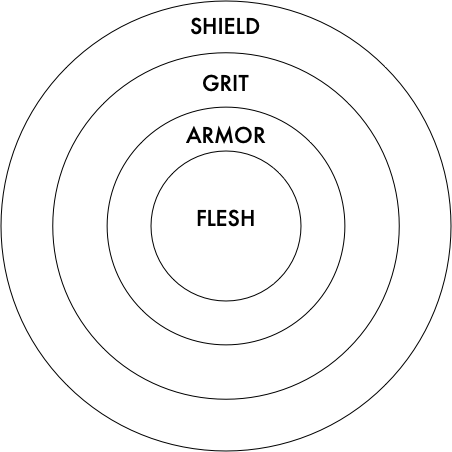
\includegraphics[scale=.3]{THE_ORDER}
  \end{center}

  \mynumlist {
    \item \mybold{Shield} : If you have a shield equipped (that is, on your arm) and take \mybold{physical damage} , you can perform the \mylink{Mighty Deed of Arms: Splinter}{combat-tactical-maneuver-splinter} (this counts as your Fight Action for the Moment; if you already took your Fight Action, you can't use this). The shield is sundered and you take no damage. Stop here.  Otherwise ...
    \item \mybold{Grit} : Subtract the damage from your Grit.  If there's any damage left over, move to Armor i.e. if I have a Grit of 4 and I take 9 damage, I have 5 damage left over and I move onto to Armor.
    \item \mybold{Armor} : If you have armor, see if it will absorb the damage.  Roll the {ud} for your armor and subtract the result from the damage.  For example, if I'm wearing chain mail (Medium armor) I roll a d8; if I rolled a 5, I'd subtract 5 from the total damage.  If there's any damage left over, move onto Flesh
    \item \mybold{Flesh} : Subtract the rest of the damage from Flesh. If you go to 0 or less Flesh, you are \mylink{Dying}{combat-dying}
  }




\mysubsection{Flesh and Grit}{combat-flesh-grit}

Flesh is your ability to withstand injury; Grit is your ability to avoid injury in the first place.  Damage affects Grit first - dodging and weaving, close calls, little nicks, stunning blows, getting worn out from the fight, etc. When Grit is gone you're too exhausted to ward off physical harm and you start taking Flesh damage.

Your starting Flesh is defined by your \FLESH.  When you start your life as an adventurer, your initial \FLESH is the \MAX of a d4, d6, d8, or d10 (the die is defined in your Trope or Species). You then roll your \VIG and, if the number on the die is higher than your initial \FLESH, your \MAX Flesh is this new number (for example, if I have a d6 \FLESH and a d8 \VIG, I start with 6 Flesh.  I then roll the d8 - if I roll a 7, my \MAX Flesh is now 7).

When you're \mylink{taking a Breather}{combat-resting-breather} or resting, you use your \FLESH to heal your \mybold{Grit} - basically patching yourself up, strapping wounds, getting yourself psyched up, that sort of thing.  

Flesh is pretty static, except for \mylink{Barbarians}{flavor-barbarian} who get to roll to see if their Flesh increases at every level.  If you're ever at a point where you're taking damage to Flesh, you're getting pretty close to \mylink{Dying}{combat-dying}.


  \mysubsection{Dying}{combat-dying}

  If your Flesh ever goes to 0 or below, you are on \mybold{Dying} .  Your Grit immediately drops to 0 if it isn't 0 already (you can't duck, dive, dodge, dip and dive while trying to hold your intestines in, right?) and your Flesh is set to 0.

  Until your Flesh is healed, you must roll a \DEATH any time you take damage.  Your Death Die depends on your \LVL.

  \mytable{X c}{
    \thead{\LVL} & \thead{Base \DEATH} \\
  }{
    1 & d3  \\
    2 & d4  \\
    3 & d6  \\
    4 & d8  \\
    5 & d10  \\
    6 & d12  \\
    7 & d16  \\
    8 & d20  \\
    9 & d24  \\    
  }

  The Death Die above are just the base. The Arbiter might start you at a lower Death Die than your level dictates if something particularly terrible happens. 

  You can't heal Grit while you are on Dying.  If you are healed above 0 Flesh (through Resting, Leechcraft, etc), you are no longer on Dying.  Your Death Die resets and you must roll on the \mylink{Wound table}{appendixa-combat-tables-wounds} as well as roll your Sanity \UD.  Note that some Wounds will prevent you from healing Grit until they are dealt with.


  \myhighlight{The Death Die}{combat-death-die}

  While you are Dying, you must \RS : \DEATH any time you take damage or do something strenuous (fighting or running counts, crawling off to a corner doesn't). If you succeed, the \DEATH moves \DCDOWN. If you fail you perish at the \mylink{top of the next Moment}{time-top-bottom} (if you're lucky, you can be healed before that happens).

  \mybold{Optional: Heinous Damage}

  If you ever take 4x your \MAX Flesh in damage, and this results in you Dying, you perish at the \mylink{top of the next Moment}{time-top-bottom} as if you had failed your \RS : \DEATH i.e. if you were a Bravo with 8 Flesh and took 32 damage, you would perish at the \mylink{top of the next Moment}{time-top-bottom}


 

  \mysection{When The Dust Settles}{combat-resting}


  \mysubsection{Taking a Breather (Minutes)}{combat-resting-breather}

  Combat takes Minutes to finish, no matter how many Moments actually occurred.  Once Combat is over, you can take a \mybold{Breather}.  Roll your \FLESH and restore that much Grit up to your \MAX (unless a Wound prevents you from doing so). Pooka can help with this process significantly. Additionally, if you are a Soldier, you may repair your Armor up to its \MAX \UD.   

  You do not need to take a Breather in a safe place, but dropping down for a nap right after you've gutted the Plague Prophet in front of his congregation may not be the hottest idea.  You can only take 1 Breather per Combat.  

  \cbreak
  
  \mysubsection{Taking a Bivouac (Hours)}{combat-resting-bivouac}
  You must take a Bivouac in a "safe" place (though this doesn't necessarily have to be in \mylink{Civilization}{civilization}).  Each time you Bivouac you must make a \UD roll of your Personal Provisions (you can share Personal Provisions with others, but you have to roll for each person).  If you don't have enough Personal Provisions, you can't get any of the effects of a Bivouac.  There's always a chance of wandering Monsters during a Bivouac (unless you have a Pooka with you)

  \mybold{If a Wound doesn't prevent you from doing so:}
  \mybullet {
    \item Restore all your Grit.  
    \item Restore \LVL Flesh.  If you're a \mylink{Barbarian}{flavor-barbarian}, restore \LVL x2 Flesh
    \item Restore 1 \UD of any \myital{one} \mylink{Intangible Stat}{intangible-stats}
    \item Restore your Armor up to its \MAX \UD
  }

  \cbreak

  \mybold{Additionally:}
  \mybullet {
    \item If you're a \mylink{Soldier}{flavor-soldier}, restore 1 \UD of Armor up to its \MAX and 1 \DEED
    \item If you're a \mylink{Barbarian}{flavor-barbarian}, restore 1 Deed \UD
    \item If you're a \mylink{Knave}{trope-knave} or a \mylink{Pooka}{species-pooka}, restore 1 Luck \UD
    \item If you're a \mylink{Sorcerer}{flavor-sorcerer}, restore 1 Blood \POOL
    \item If you're a \mylink{Leech}{flavor-leech}, reset any negative modifiers to Knowledge
    \item If you're a \mylink{Mystic}{flavor-mystic}, restore 1 Grace \POOL
    \item If you're a \mylink{Witch}{flavor-witch}, restore 1 Mojo \UD
    \item If you're a \mylink{Spriggan}{species-spriggan}, restore 1 Remembrance die \UD
  }


  \mysubsection{Longer Rests}{civilization-resting-longer-rests}
  As your injuries mount and your experience grows,  you may find you need to take a longer rest.  Longer rests require \mylink{Civilization}{civilization}.  If you rest for a Days in Civilization, this is a Sojourn; if you rest for Weeks, this is a Sabbatical. 

} %end